\let\negmedspace\undefined
\let\negthickspace\undefined
\documentclass[journal]{IEEEtran}
\usepackage[a5paper, margin=10mm, onecolumn]{geometry}
\usepackage{lmodern} % Ensure lmodern is loaded for pdflatex
\usepackage{tfrupee} % Include tfrupee package

\setlength{\headheight}{1cm} % Set the height of the header box
\setlength{\headsep}{0mm}     % Set the distance between the header box and the top of the text

\usepackage{gvv-book}
\usepackage{gvv}
\usepackage{cite}
\usepackage{amsmath,amssymb,amsfonts,amsthm}
\usepackage{algorithmic}
\usepackage{graphicx}
\usepackage{textcomp}
\usepackage{xcolor}
\usepackage{txfonts}
\usepackage{listings}
\usepackage{enumitem}
\usepackage{mathtools}
\usepackage{gensymb}
\usepackage{comment}
\usepackage[breaklinks=true]{hyperref}
\usepackage{tkz-euclide} 
\usepackage{listings}
\usepackage{gvv}                                        
\def\inputGnumericTable{}                                 
\usepackage[latin1]{inputenc}                                
\usepackage{color}                                            
\usepackage{array}                                            
\usepackage{longtable}                                       
\usepackage{calc}                                             
\usepackage{multirow}                                         
\usepackage{hhline}                                           
\usepackage{ifthen}                                           
\usepackage{lscape}
\begin{document}

\bibliographystyle{IEEEtran}
\vspace{3cm}

\title{4.4.2.7}
\author{EE24BTECH11024 - Abhimanyu Koushik}
% \maketitle
% \newpage
% \bigskip
{\let\newpage\relax\maketitle}
Question:\\
Find the equation of circle which passes through the points $\myvec{2\\3}$ and $\myvec{4\\5}$ and the centre lies on the straight line $y-4x+3=0$
\begin{table}[h!]    
  \centering
  \begin{tabular}[12pt]{ |c|c|c|}
    \hline
    \textbf{Symbol} & \textbf{Value} & \textbf{Description} \\
    \hline
    $\vec{A}$ & \myvec{6\\5} & First point\\
    \hline 
    $\vec{B}$ & \myvec{-4\\3} & Second point\\
    \hline
    $\vec{Y}$ & \myvec{0\\$y$} & Point on Y-Axis equidistant from A and B\\
    \hline
    \end{tabular}

  \caption{Variables Used}
  \label{tab1-1.9-6}
\end{table}\\
Let the equation of circle be $\norm{\vec{x}}^2+2\vec{u}^\top\vec{x}+f=0$ where $\vec{u}=-\vec{c}$, $f=\norm{\vec{u}}^2-r^2$ and the equation of diameter be $\vec{n}^\top\vec{x}=c$. Then
\begin{align}
\norm{\vec{x_1}}^2+2\vec{u}^\top\vec{x_1}+f&=0\\
\norm{\vec{x_2}}^2+2\vec{u}^\top\vec{x_2}+f&=0\\
-\vec{u}^\top\vec{n}&=c
\end{align}
These equations can be written as 
\begin{align}
2\vec{x_1}^\top\vec{u}+f&=-\norm{\vec{x_1}}^2\\
2\vec{x_2}^\top\vec{u}+f&=-\norm{\vec{x_2}}^2\\
\vec{n}^\top\vec{u}&=-c
\end{align}
Turning them into matrix form gives
\begin{align}
\myvec{2\vec{x_1}^\top & 1\\2\vec{x_2}^\top & 1\\ \vec{n}^\top & 0}\myvec{\vec{u}\\f}&=-\myvec{\norm{\vec{x_1}}^2\\\norm{\vec{x_2}}^2\\c}\\
\end{align}
Given the equation of diameter
\begin{align}
y-4x+3&=0\\
\myvec{-4 & 1}\myvec{x\\y}&=-3\\
\myvec{-4\\1}^\top\vec{x}&=-3\\
\vec{n}&=\myvec{-4\\1}\\
c&=-3
\end{align}
Given $\vec{x_1}=\myvec{2\\3}$, $\vec{x_2}=\myvec{4\\5}$. substituting into the matrix equation gives
\begin{align}
\myvec{4 & 6 & 1\\8 & 10 & 1\\-4 & 1 & 0}\myvec{\vec{u}\\f}=\myvec{-13\\-41\\3}
\end{align}
The Augmented matrix is 
\begin{align}
\myvec{4 & 6 & 1 & -13\\8 & 10 & 1 & -41\\-4 & 1 & 0 & 3}
\end{align}
Solving the matrix equation
\begin{align}
\myvec{4 & 6 & 1 & -13\\8 & 10 & 1 & -41\\-4 & 1 & 0 & 3}\xleftrightarrow[]{R_3 \leftarrow R_1+R_3}\myvec{4 & 6 & 1 & -13\\8 & 10 & 1 & -41\\0 & 7 & 1 & -10}\\
\xleftrightarrow[]{R_2 \leftarrow R_2-2R_1}\myvec{4 & 6 & 1 & -13\\0 & -2 & -1 & -15\\0 & 7 & 1 & -10}\\
\xleftrightarrow[]{R_3 \leftarrow 2R_3+7R_2}\myvec{4 & 6 & 1 & -13\\0 & -2 & -1 & -15\\0 & 0 & -5 & -125}\\
\xleftrightarrow[]{R_3 \leftarrow \frac{R_3}{-5}}\myvec{4 & 6 & 1 & -13\\0 & -2 & -1 & -15\\0 & 0 & 1 & 25}\\
\xleftrightarrow[]{R_2 \leftarrow R_2+R_3}\myvec{4 & 6 & 1 & -13\\0 & -2 & 0 & 10\\0 & 0 & 1 & 25}\\
\xleftrightarrow[]{R_2 \leftarrow \frac{R_2}{-2}}\myvec{4 & 6 & 1 & -13\\0 & 1 & 0 & -5	\\0 & 0 & 1 & 25}\\
\xleftrightarrow[]{R_1 \leftarrow R_1-R_3}\myvec{4 & 6 & 0 & -38\\0 & 1 & 0 & -5\\0 & 0 & 1 & 25}\\
\xleftrightarrow[]{R_1 \leftarrow R_1-6R_2}\myvec{4 & 0 & 0 & -8\\0 & 1 & 0 & -5\\0 & 0 & 1 & 25}\\
\xleftrightarrow[]{R_1 \leftarrow \frac{R_1}{4}}\myvec{1 & 0 & 0 & -2\\0 & 1 & 0 & -5\\0 & 0 & 1 & 25}
\end{align}
The value of u and f is 
\begin{align}
\vec{u}&=\myvec{-2\\-5}\\
f&=25
\end{align}
The centre and radius of circle is
\begin{align}
\vec{c}&=\myvec{2\\5}\\
r&=\sqrt{2^2+5^2-25}\\
r&=2
\end{align}
The equation of circle is $\norm{\vec{x}}^2-2\myvec{2 & 5}\vec{x}+25=0$
\begin{figure}[h!]
   \centering
   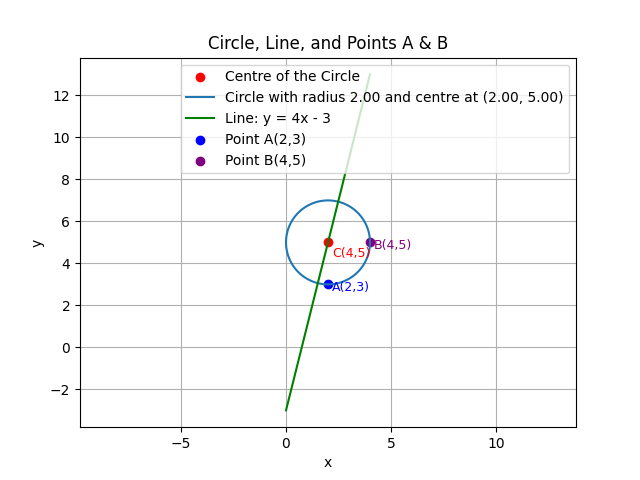
\includegraphics[width = 1\linewidth]{figs/fig.png}
   \caption{The circle which satisfies the conditions}
   \label{stemplot}
\end{figure}
\end{document}
